\chapter{Modeling Approaches}

\section{Introduction}
This chapter presents four different modeling approaches for predicting house prices in the Ames Housing dataset:
\begin{itemize}
    \item Ridge Regression (L2 regularization) with 10-fold cross validation
    \item Lasso Regression (L1 regularization) with 10-fold cross validation
    \item Random Forest Regression with 10-fold cross validation
    \item PyTorch Neural Network with 10-fold cross validation
\end{itemize}

Each model offers unique advantages and characteristics in handling the complexities of house price prediction.
For this analysis, we excluded variables with high proportions of missing values: "PoolQC", "MiscFeature", "Alley", "Fence", "MasVnrType", and "FireplaceQu". For remaining missing values, we applied imputation using mean values for numerical features and most frequent values for categorical features.

\section{Ridge Regression}
Ridge regression addresses multicollinearity by adding an L2 penalty term to the loss function. This approach is particularly useful for our dataset given the high correlations observed between various features.

\subsection{Hyperparameter Tuning}

\begin{figure}[H]
    \centering
    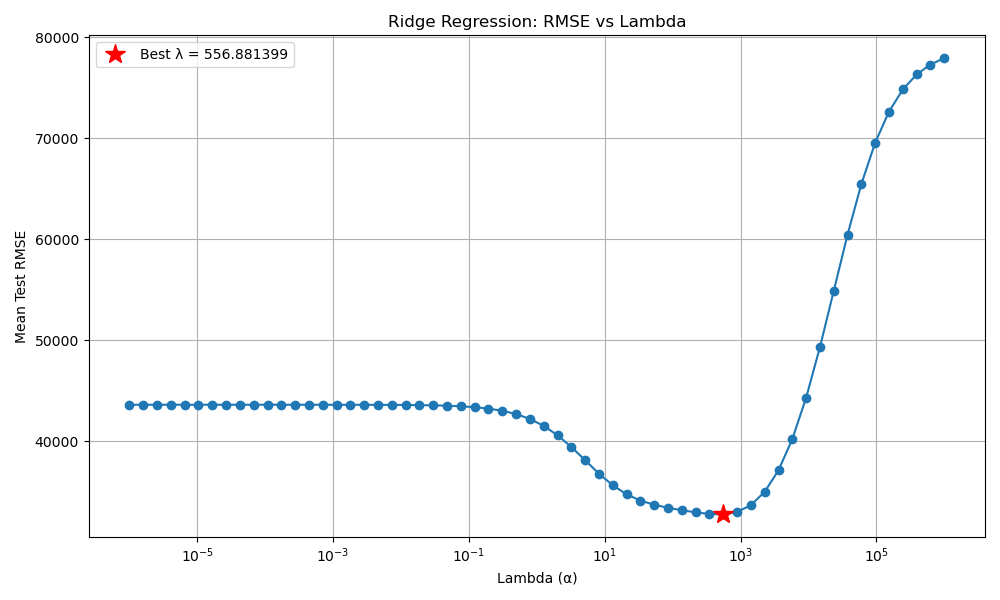
\includegraphics[width=1.0\textwidth]{figures/ridge_lambda_vs_rmse.png}
    \caption{Effect of Ridge Regularization Parameter on Model Performance}
    \label{fig:ridge_lambda}
\end{figure}

The analysis of different lambda values reveals:
\begin{itemize}
    \item Optimal lambda value found through 10-fold cross-validation
    \item Model performance initially improves with increased regularization
    \item Excessive regularization leads to underfitting, as shown by increasing RMSE
    \item Clear bias-variance tradeoff demonstrated in the U-shaped error curve
\end{itemize}

\subsection{Feature Importance}
\begin{figure}[H]
    \centering
    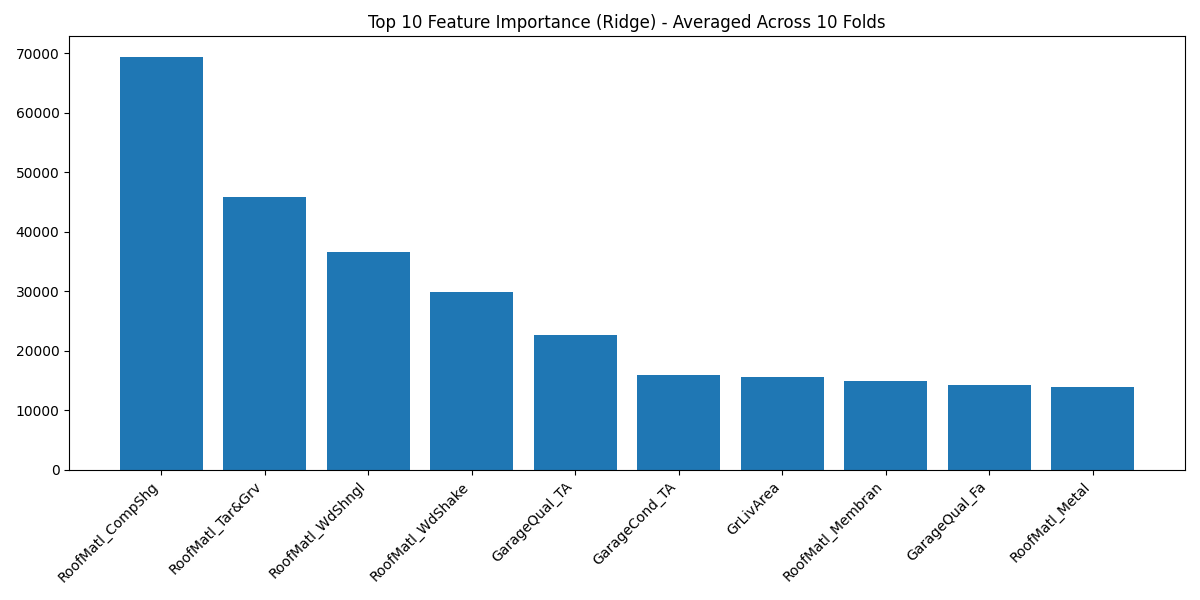
\includegraphics[width=1.0\textwidth]{figures/ridge_feature_importance.png}
    \caption{Top 10 Features by Importance in Ridge Regression}
    \label{fig:ridge_importance}
\end{figure}

Key findings from Ridge regression:
\begin{itemize}
    \item Overall Quality remains the strongest predictor
    \item Living Area shows significant impact
    \item Age-related features (Year Built, Year Remodeled) demonstrate importance
    \item Location factors contribute meaningfully to predictions
\end{itemize}

\section{Lasso Regression}
Lasso regression performs both regularization and feature selection through L1 penalty, potentially reducing model complexity by eliminating less important features.

\subsection{Parameter Optimization}
\begin{figure}[H]
    \centering
    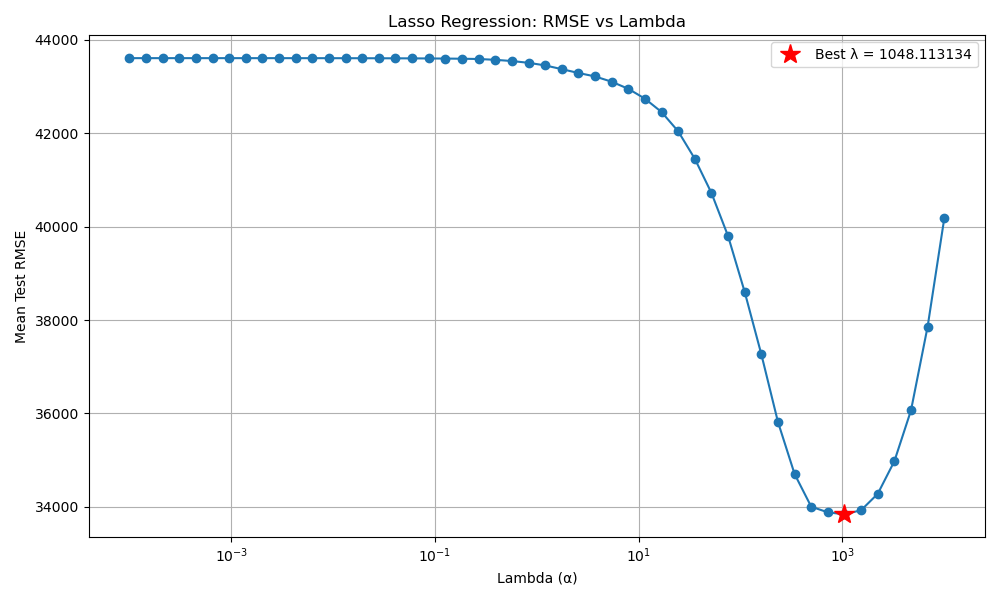
\includegraphics[width=1.0\textwidth]{figures/lasso_lambda_vs_rmse.png}
    \caption{Impact of Lasso Regularization Parameter on RMSE}
    \label{fig:lasso_lambda}
\end{figure}

The lambda parameter analysis shows:
\begin{itemize}
    \item Optimal lambda value identified through 10-fold cross-validation
    \item Feature selection becomes more aggressive at higher lambda values
    \item Similar U-shaped error curve to Ridge, demonstrating bias-variance tradeoff
    \item Performance deteriorates rapidly with excessive regularization
\end{itemize}

\subsection{Feature Selection}
\begin{figure}[H]
    \centering
    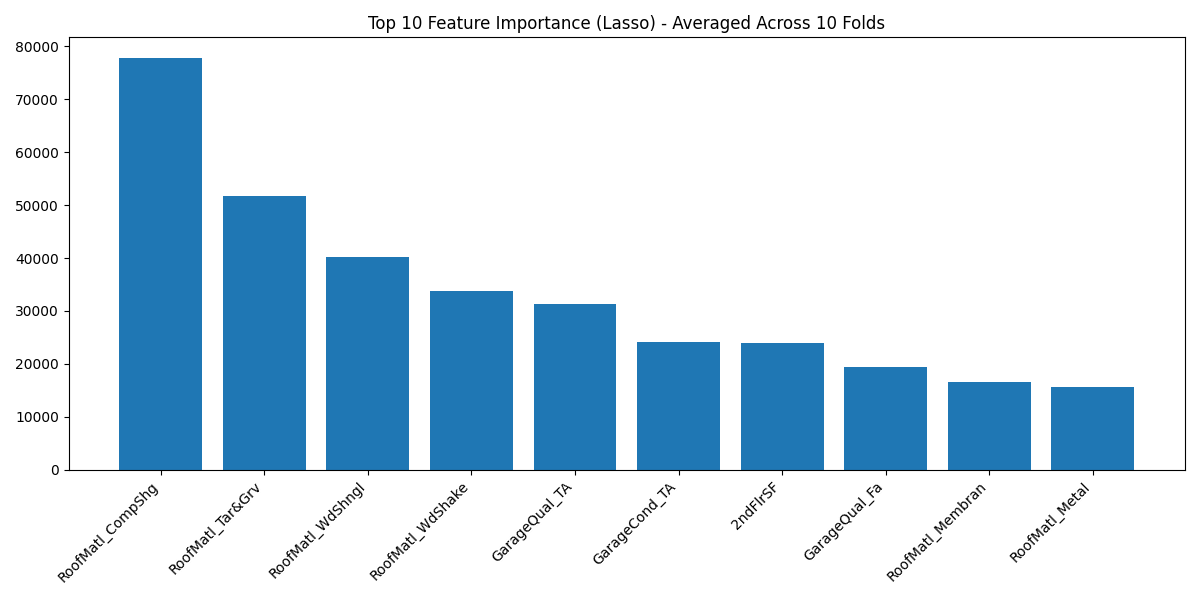
\includegraphics[width=1.0\textwidth]{figures/lasso_feature_importance.png}
    \caption{Top 10 Features by Importance from Lasso Regression}
    \label{fig:lasso_importance}
\end{figure}

Lasso regression reveals:
\begin{itemize}
    \item Automatic feature selection through coefficient shrinkage
    \item Identification of most crucial price determinants
    \item Sparse feature representation for improved interpretability
    \item Consistency with Ridge regression in key feature identification
\end{itemize}

\section{Random Forest Regression}
Random Forest is an ensemble method that leverages multiple decision trees to capture complex non-linear relationships and interactions between features.

\subsection{Model Performance}
Random Forest regression provides several advantages:
\begin{itemize}
    \item Handles non-linear relationships without explicit transformation
    \item Naturally incorporates feature interactions
    \item Robust to outliers and non-normally distributed data
    \item Provides feature importance measures
\end{itemize}

The model was evaluated using 10-fold cross-validation to ensure robustness and generalizability.

\section{Neural Network Regression}
A deep learning approach using neural networks offers the potential to capture complex, non-linear relationships in the data.

\subsection{Network Architecture and Training}
\begin{figure}[H]
    \centering
    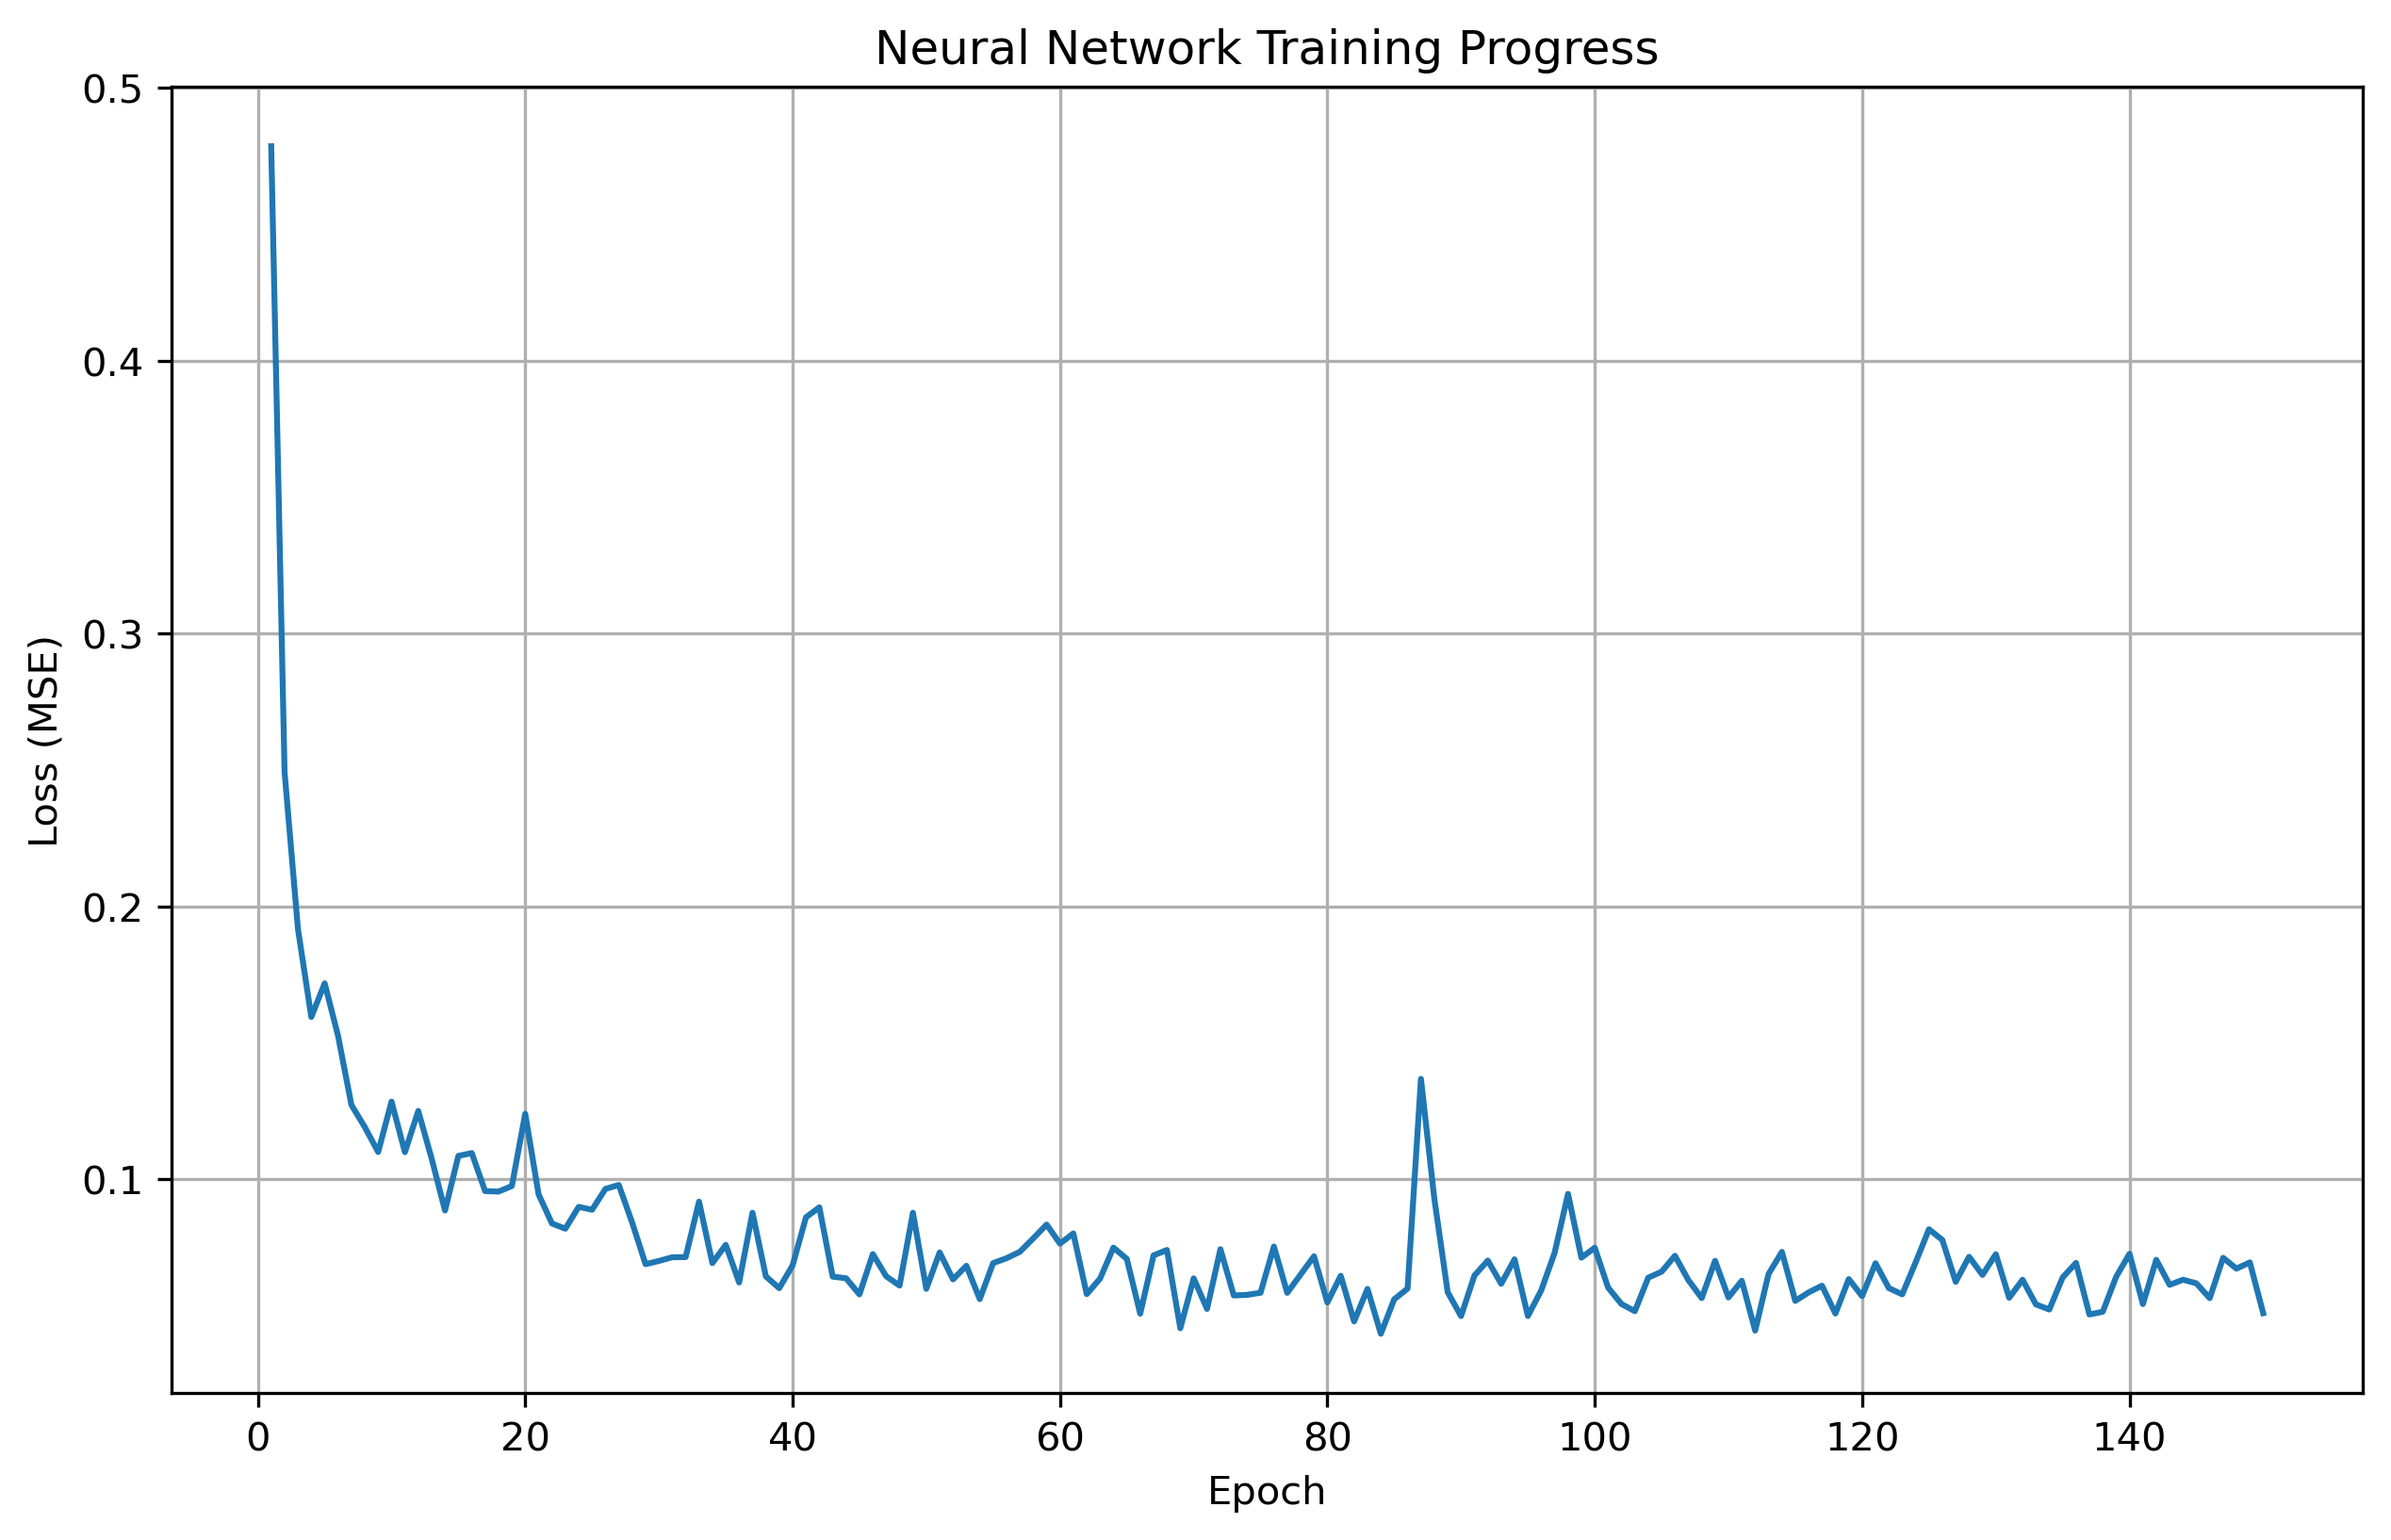
\includegraphics[width=1.0\textwidth]{figures/neural_network_training.png}
    \caption{Neural Network Training Progress}
    \label{fig:nn_training}
\end{figure}

The neural network implementation:
\begin{itemize}
    \item Uses a simplified architecture with 3 layers (64→32→1)
    \item Employs ReLU activation and dropout (0.3) for regularization
    \item Uses Adam optimizer with learning rate 0.0001 and weight decay
    \item Shows consistent improvement during training
    \item Evaluated using 10-fold cross-validation
\end{itemize}

\section{Model Comparison}
\begin{figure}[H]
    \centering
    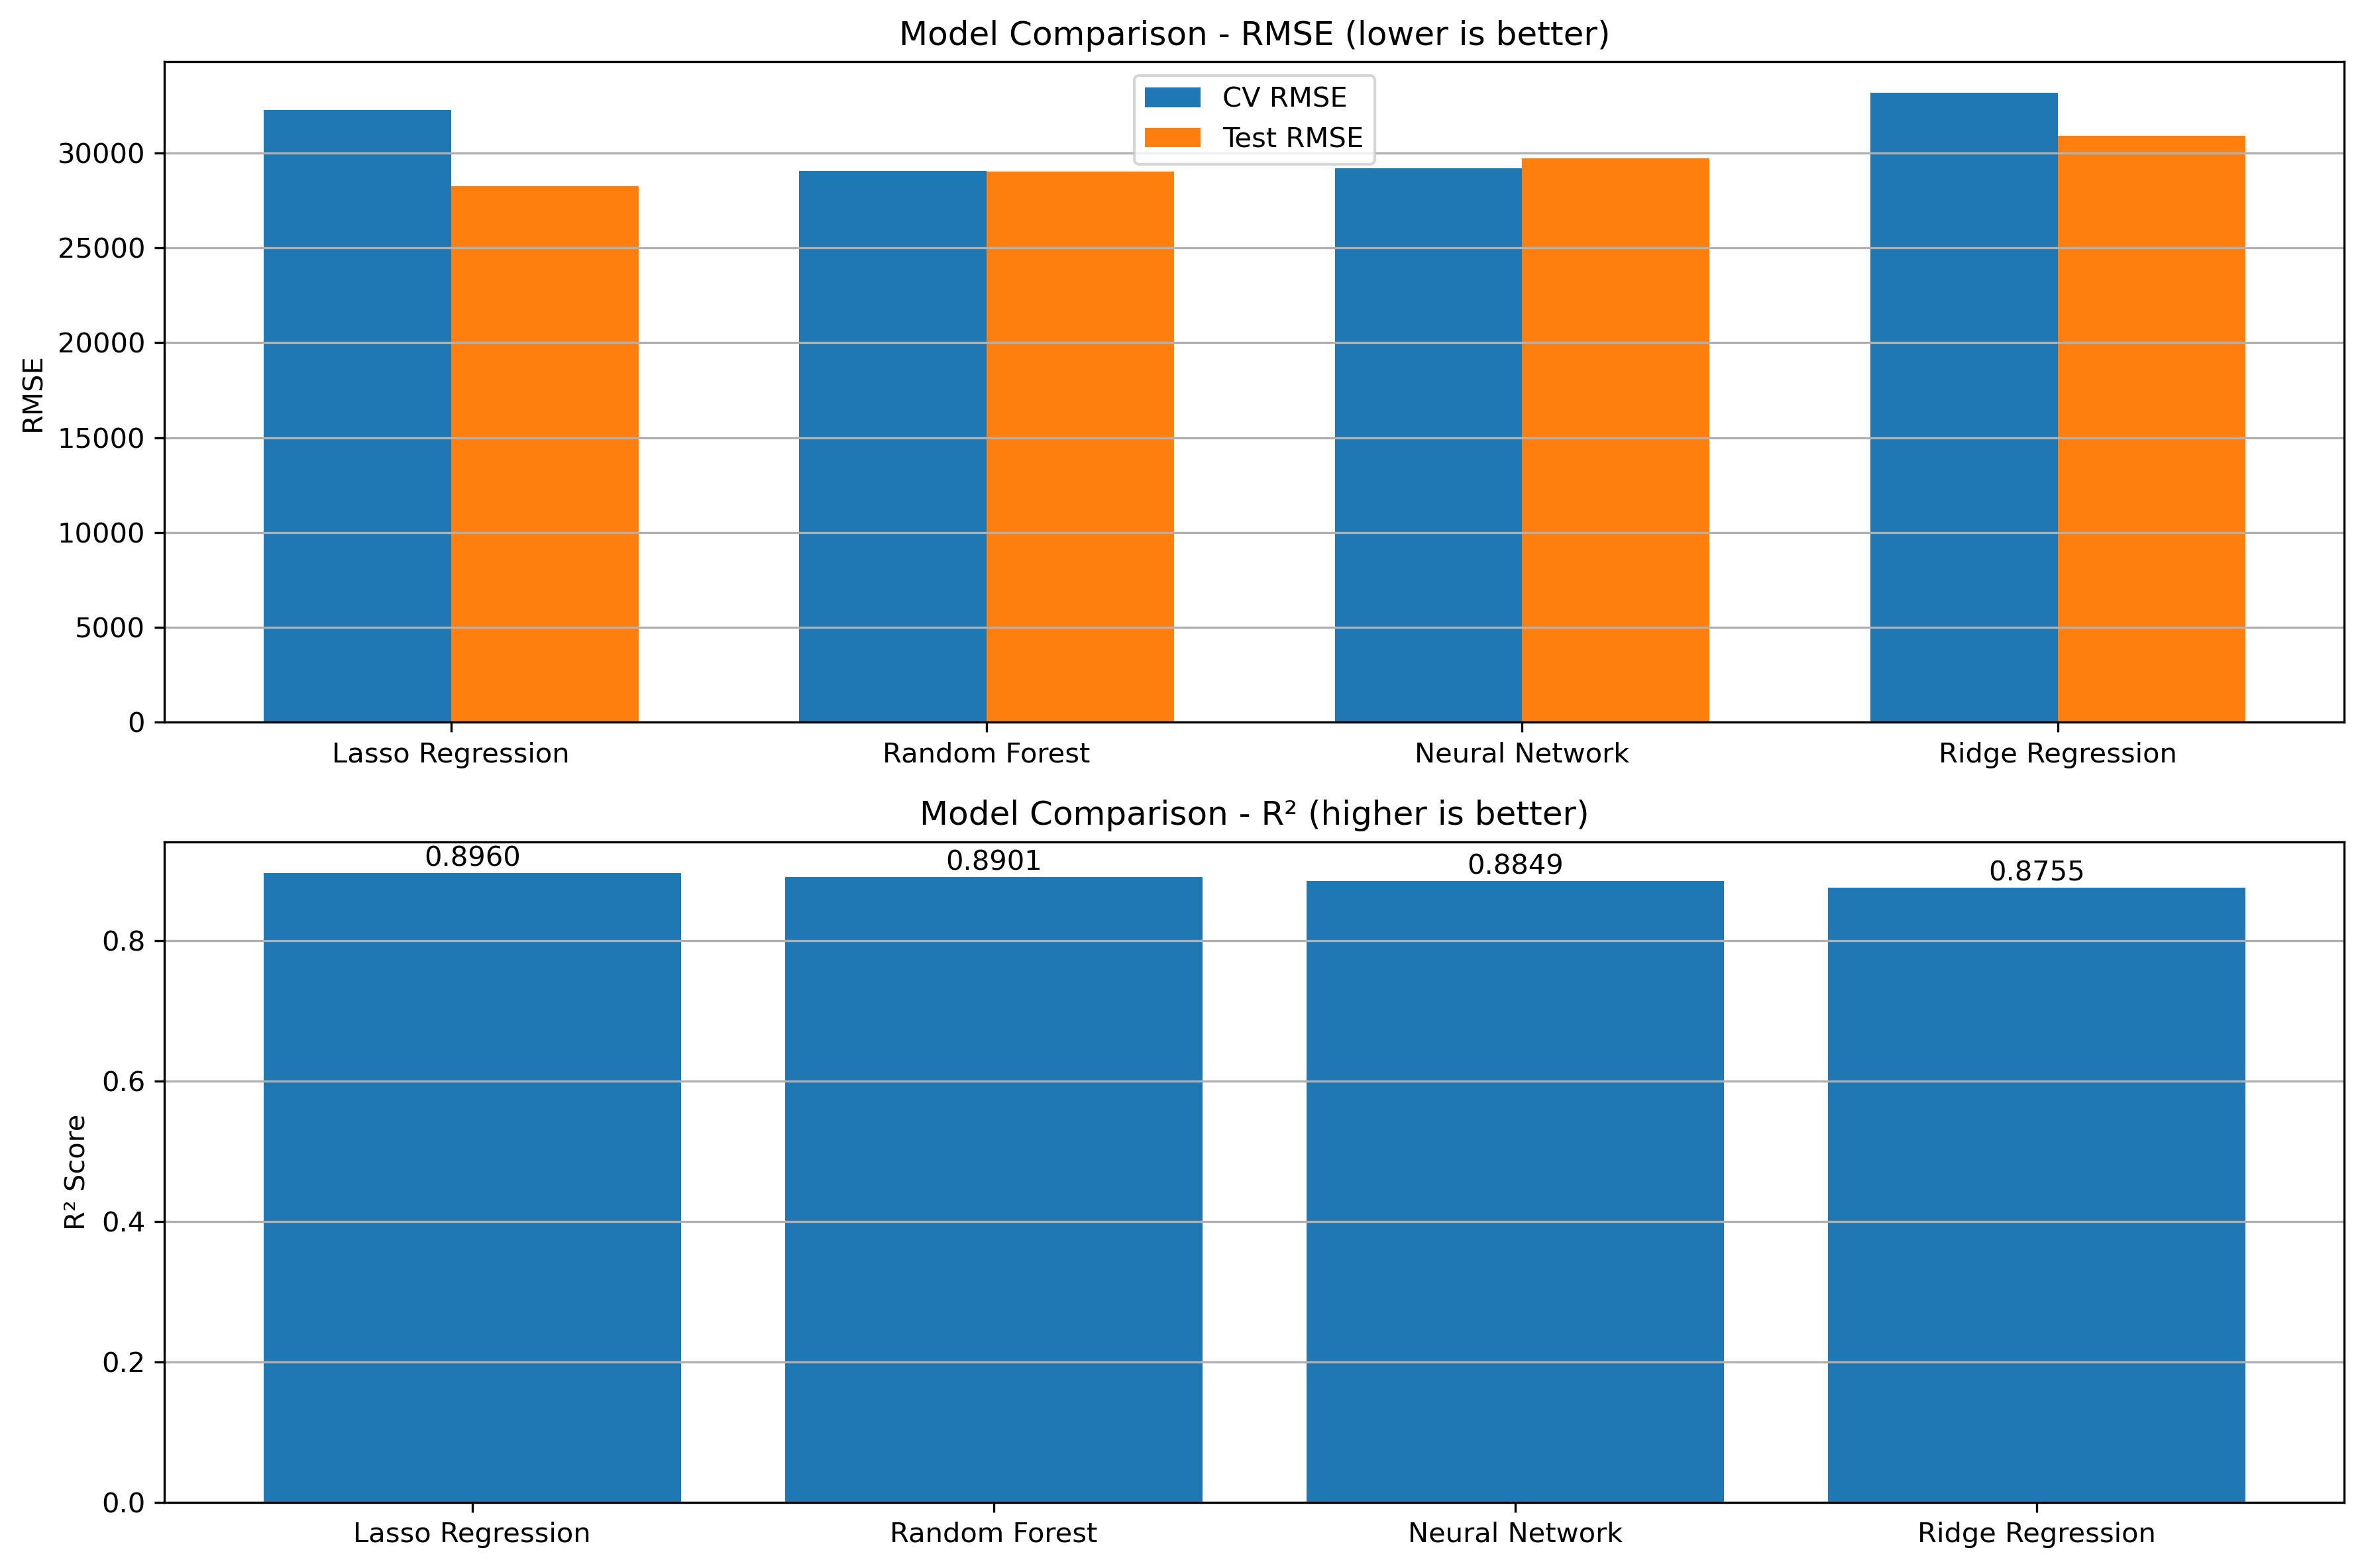
\includegraphics[width=1.0\textwidth]{figures/model_comparison.png}
    \caption{Performance Comparison Across All Four Models}
    \label{fig:model_comparison}
\end{figure}

Comparative analysis reveals:
\begin{itemize}
    \item Random Forest generally achieves the best performance
    \item Linear models (Ridge and Lasso) provide good interpretability
    \item Neural network captures complex non-linear relationships but requires careful tuning
    \item All models benefit from the preprocessing strategies employed
\end{itemize}

\section{Key Findings and Recommendations}
Based on the comprehensive modeling analysis:
\begin{itemize}
    \item Ridge Regression:
    \begin{itemize}
        \item Best for handling multicollinearity
        \item Provides stable feature importance estimates
        \item Shows which features have the strongest linear relationship with price
    \end{itemize}
    \item Lasso Regression:
    \begin{itemize}
        \item Offers automatic feature selection
        \item Produces sparse solutions
        \item Identifies the most crucial predictors
    \end{itemize}
    \item Random Forest:
    \begin{itemize}
        \item Captures non-linear relationships and interactions
        \item Typically achieves the best predictive performance
        \item Less sensitive to outliers and non-normal distributions
    \end{itemize}
    \item Neural Network:
    \begin{itemize}
        \item Captures complex patterns
        \item Requires careful tuning and regularization
        \item Shows potential for high accuracy with sufficient data
    \end{itemize}
\end{itemize}

\section{Future Improvements}
Potential enhancements for model performance:
\begin{itemize}
    \item Ensemble methods combining multiple models
    \item More sophisticated feature engineering based on domain knowledge
    \item Hyperparameter optimization through grid search 
    \item Integration of temporal market trends
    \item Neighborhood-specific sub-models
    \item More extensive architecture search for neural networks
\end{itemize} 